%!TEX root = ./main.tex
\begin{appendices}
\appendix

\chapter{Data sheets}

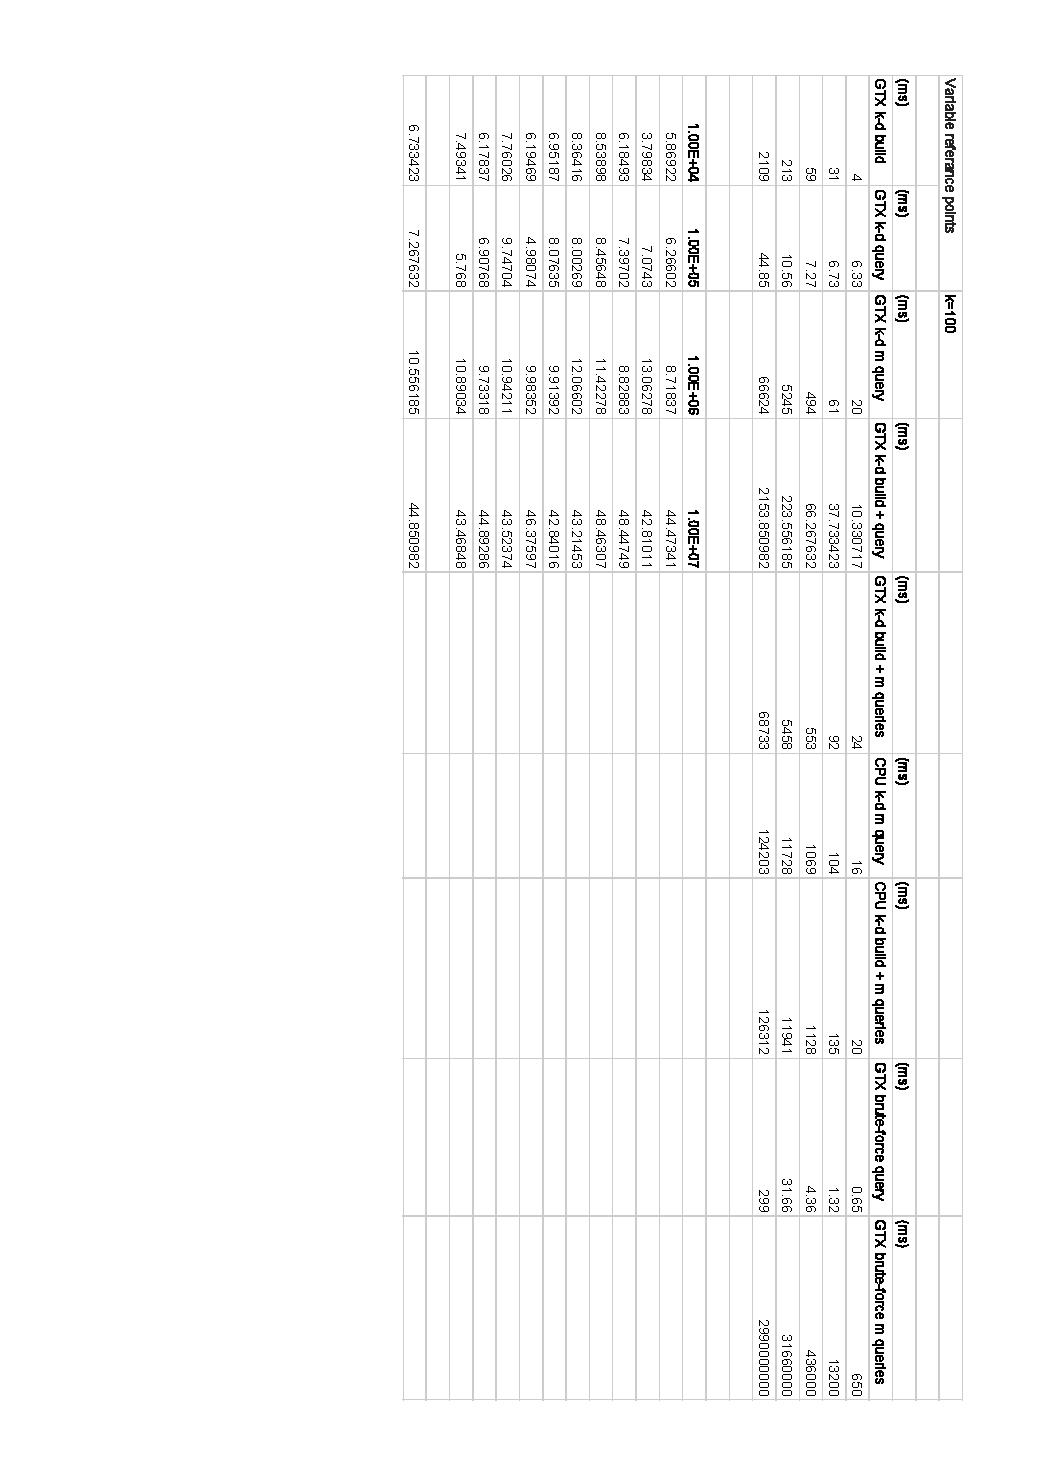
\includepdf[fitpaper=true, scale=1, noautoscale]{../gfx/data_sheet_variable_m.pdf}
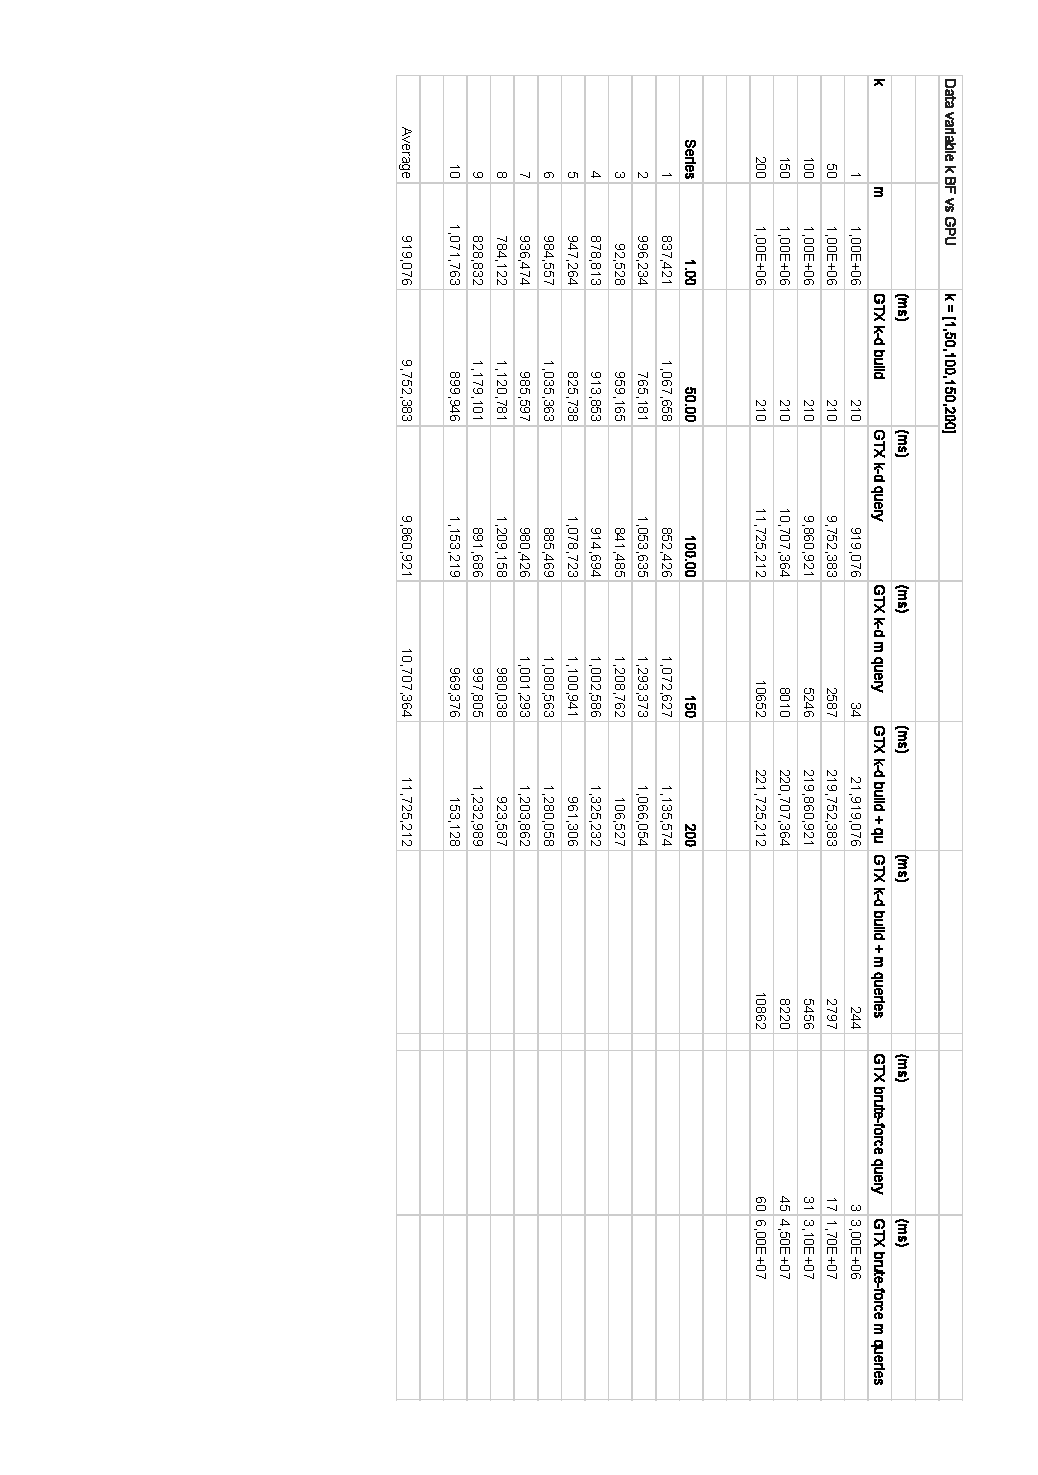
\includepdf[fitpaper=true, scale=1, noautoscale]{../gfx/data_sheet_variable_k.pdf}

% section  (end)

\chapter{Source code documentation}

\section{Api documentation} % (fold)
\label{sec:api_documentation}

% section api_documentation (end)
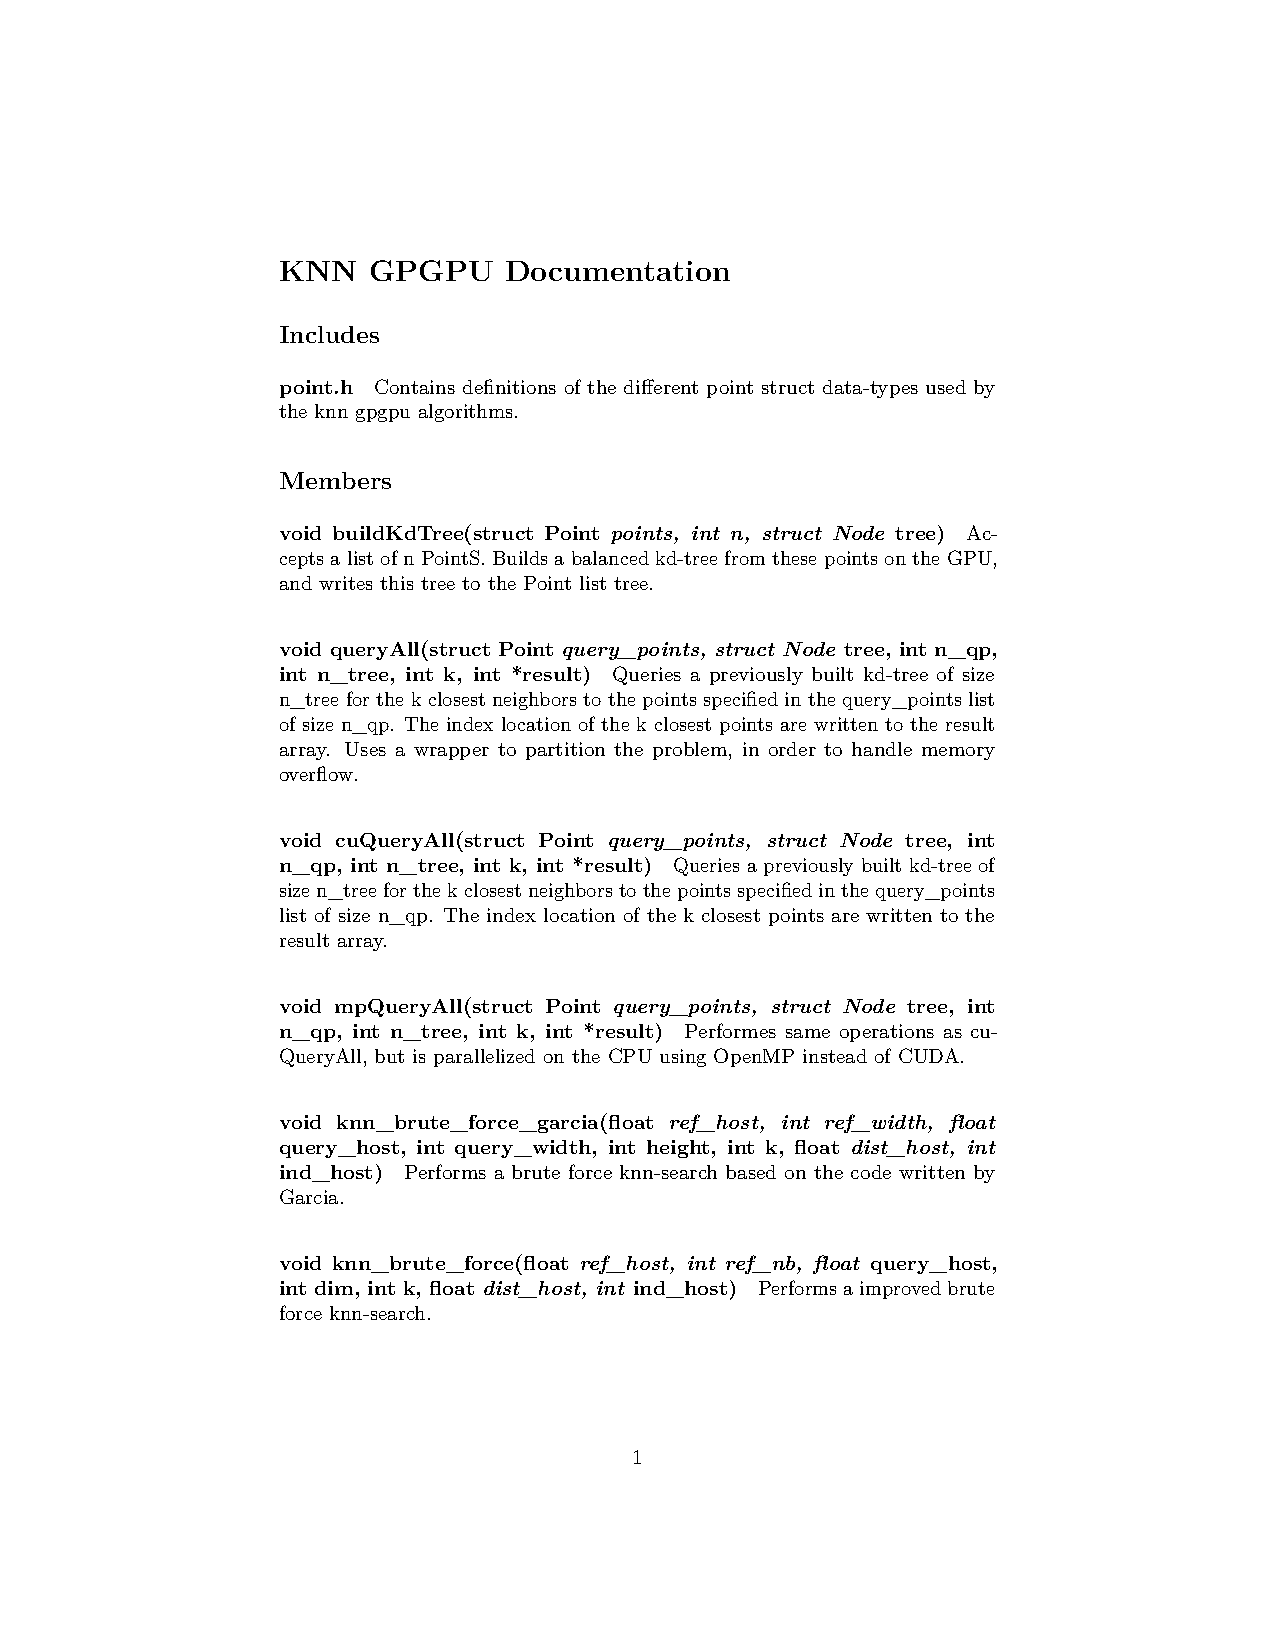
\includepdf[fitpaper=true, pages={1,2}, scale=1, noautoscale]{../gfx/api_documentation.pdf}

\section{Installation instructions} % (fold)
\label{sec:installation_instructions}
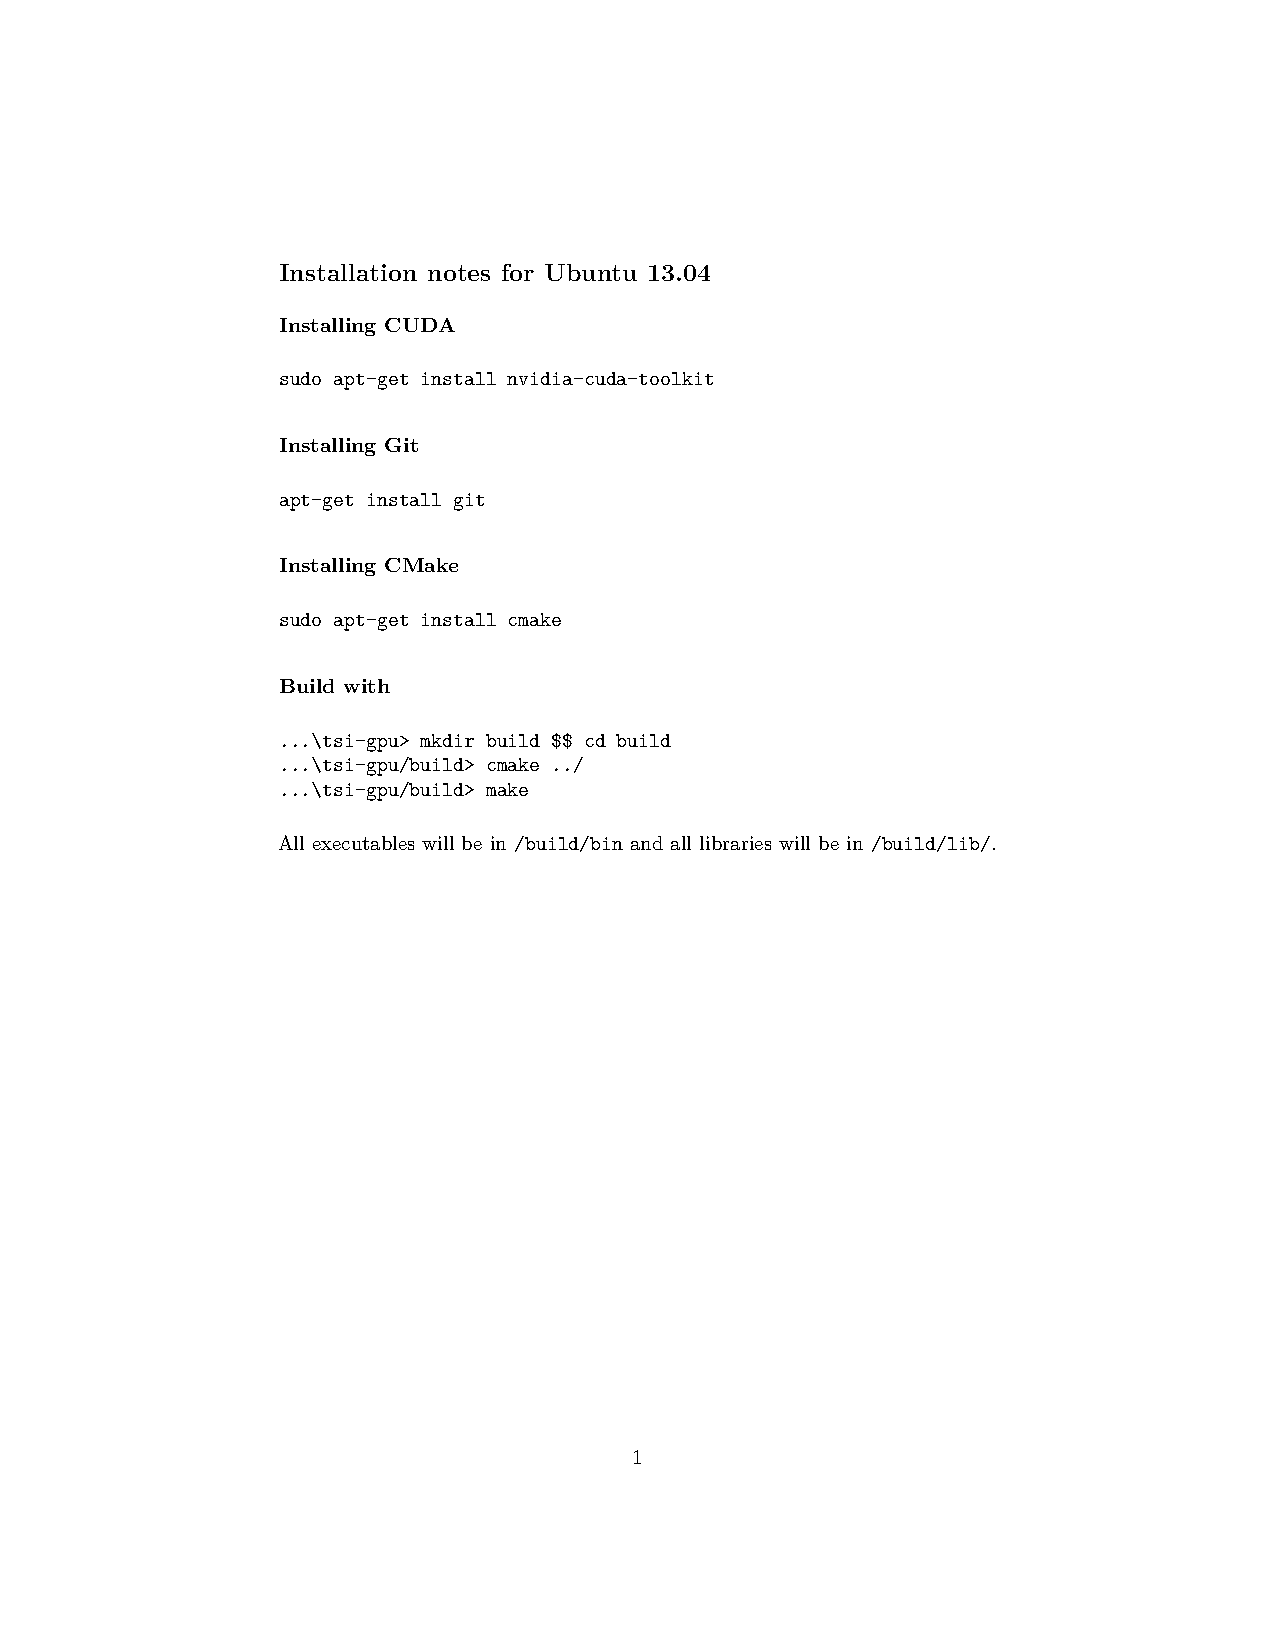
\includepdf[fitpaper=true, pages={1,2,3}, scale=1, noautoscale]{../gfx/instructions.pdf}


% section installation_instructions (end)


\chapter{Source code}

\section{API header} % (fold)
\label{sec:api_header}

\lstinputlisting[language=C,breaklines=true]{../../include/knn_gpgpu.h}

% section api_header (end)

\section{Brute Force} % (fold)
\label{sec:brute_force_garcia}

\lstinputlisting[language=C,breaklines=true]{../../src/kNN/data_types.h}


\subsection{Bitonic sort version} % (fold)
\label{sub:bitonic_force}

\lstinputlisting[language=C,breaklines=true]{../../src/kNN/brute-force/kNN-brute-force.cuh}
\lstinputlisting[language=C,breaklines=true]{../../src/kNN/brute-force/kNN-brute-force.cu}

\subsection{min-reduce version} % (fold)
\label{sub:min_reduce}
\lstinputlisting[language=C,breaklines=true]{../../src/kNN/brute-force/kNN-brute-force-reduce.cuh}
\lstinputlisting[language=C,breaklines=true]{../../src/kNN/brute-force/kNN-brute-force-reduce.cu}
\lstinputlisting[language=C,breaklines=true]{../../src/kNN/brute-force/reduction-mod.cuh}
\lstinputlisting[language=C,breaklines=true]{../../src/kNN/brute-force/reduction-mod.cu}
% subsection min_reduce (end)
% subsection bitonic_force (end)


% section brute_force_garcia (end)
\section{k-d tree build} % (fold)
\label{sec:k_d_tree_build}
\lstinputlisting[language=C,breaklines=true]{../../src/kNN/point.h}
\lstinputlisting[language=C,breaklines=true]{../../src/kNN/stack.h}

% section k_d_tree_build (end)
\subsection{Radix select} % (fold)
\label{sec:radix_select}

\lstinputlisting[language=C,breaklines=true]{../../src/kNN/kd-tree/radix-select.cuh}
\lstinputlisting[language=C,breaklines=true]{../../src/kNN/kd-tree/radix-select.cu}

% section radix_select (end)
 \subsection{Parallel quick select} % (fold)
 \label{sec:parallel_quick_select}

\lstinputlisting[language=C,breaklines=true]{../../src/kNN/kd-tree/quick-select.cuh}
\lstinputlisting[language=C,breaklines=true]{../../src/kNN/kd-tree/quick-select.cu}

 % section parallel_quick_select (end)

\subsection{Multiple radix select} % (fold)
\label{sec:multiple_radix_select}

\lstinputlisting[language=C,breaklines=true]{../../src/kNN/kd-tree/multiple-radix-select.cuh}
\lstinputlisting[language=C,breaklines=true]{../../src/kNN/kd-tree/multiple-radix-select.cu}
% section multiple_radix_select (end)
\subsection{Parallel k-d tree build} % (fold)
\label{sec:paralell_k_d_tree_build}

\lstinputlisting[language=C,breaklines=true]{../../src/kNN/kd-tree/kd-tree-build.cuh}
\lstinputlisting[language=C,breaklines=true]{../../src/kNN/kd-tree/kd-tree-build.cu}
% section paralell_k_d_tree_build (end)

\section{k-d tree search} % (fold)
\label{sec:k_d_tree_search}

\subsection{CUDA k-d tree search} % (fold)
\label{sec:cuda_k_d_tree_search}

\lstinputlisting[language=C,breaklines=true]{../../src/kNN/kd-tree/cu-kd-search.cuh}
\lstinputlisting[language=C,breaklines=true]{../../src/kNN/kd-tree/cu-kd-search.cu}
% section cuda_k_d_tree_search (end)

\subsubsection{k-d tree split wrapper} % (fold)
 \label{sub:wrapper}
 
\lstinputlisting[language=C,breaklines=true]{../../src/common/utils.cuh}
\lstinputlisting[language=C,breaklines=true]{../../src/common/utils.cu}
\lstinputlisting[language=C,breaklines=true]{../../src/kNN/kd-tree/kd-search.cuh}
\lstinputlisting[language=C,breaklines=true]{../../src/kNN/kd-tree/kd-search.cu}
 % subsection wrapper (end)


\subsection{OpenMP k-d tree search} % (fold)
\label{sec:open_mp_k_d_tree_search}


\lstinputlisting[language=C,breaklines=true]{../../src/kNN/kd-tree/kd-search-openmp.cuh}
\lstinputlisting[language=C,breaklines=true]{../../src/kNN/kd-tree/kd-search-openmp.cu}
% section k_d_tree_search_das_openmp (end)
% section k_d_tree_search (end)
\end{appendices}
